\subsection{Methods}
For the second week, I added a depth-first minimax agent to the tic-tac-toe program. In its original version, nothing was optimized, and the agent would expand the entire minimax tree. Then, as this program took around 40 seconds per game, three optimizations were successively added upon the program.

The first optimization was eliminating the \texttt{deepcopy} method, where the board was originally copied for each expansion. Instead, moves were made in-place on the board, and were undone when that branch had been checked.

On top of this, I began caching board states. Hence, if a node had already been checked and cached, it would not be expanded. This approach recognizes that the configuration of nodes is truly a graph (not a tree), as there are different permutations of moves that lead to the same state. The cache was cleared at the end of each game.

The final optimization was prioritizing early wins. Instead of scoring each leaf node (end-of-game node) simply by whether it was a win/loss/draw (which were scored 1/-1/0), this method would divide the original score by the depth of the leaf node, hence assigning greater priority higher nodes. The intent here is to end the game as early as possible while still attaining the same result (in terms of a win/loss/draw).

\subsection{Results}

\subsubsection{Minimax vs. Minimax}
With two minimax agents, no randomness was involved, and hence the game was completely deterministic, ending in configuration below (a draw).
\[
    \begin{array}{c|c|c}
        \text{x} & \text{x} & \text{o}\\
        \hline
        \text{o} & \text{o} & \text{x}\\
        \hline
        \text{x} & \text{o} & \text{x}\\
    \end{array}    
\]
It should be noted that, at the first move, there were multiple moves scored \texttt{0} in minimax, but the first (top left) was chosen. This even occured when spots were chosen by priority of depth, as all draws will have depth 9 (a draw is always on a full board).

The two log-scaled graphs below show the results, over 10 games in each of the successive optimizations, of average runtime and states visited. Note that each successive optimization was applied on top of the previous.
\begin{center}
    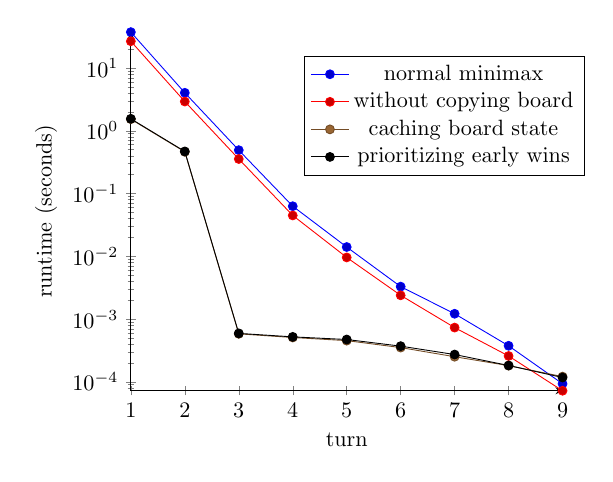
\begin{tikzpicture}[scale=.8]
        \begin{axis}[
            legend style={at={(.4,.6)},anchor=south west},
            axis lines = left,
            xlabel = turn,
            xtick = {0, 1, 2, 3, 4, 5, 6, 7, 8, 9},
            ymode = log,
            ylabel = runtime (seconds),
        ]
        \addplot+[
            mark=*,
        ] plot coordinates{
            (1,37.328725)
            (2,4.028346)
            (3,0.490918)
            (4,0.062810)
            (5,0.014050)
            (6,0.003286)
            (7,0.001214)
            (8,0.000375)
            (9,0.000093)
        };
        \addlegendentry{normal minimax}
        \addplot+[
            mark=*,
        ] plot coordinates{
            (1,26.668035)
            (2,2.922236)
            (3,0.354789)
            (4,0.044750)
            (5,0.009588)
            (6,0.002387)
            (7,0.000731)
            (8,0.000258)
            (9,0.000072)
        };
        \addlegendentry{without copying board}
        \addplot+[
            mark=*,
        ] plot coordinates{
            (1,1.530653)
            (2,0.462433)
            (3,0.000581)
            (4,0.000508)
            (5,0.000453)
            (6,0.000351)
            (7,0.000251)
            (8,0.000181)
            (9,0.000121)
        };
        \addlegendentry{caching board state}
        \addplot+[
            mark=*,
        ] plot coordinates{
            (1,1.551102)
            (2,0.468198)
            (3,0.000591)
            (4,0.000520)
            (5,0.000472)
            (6,0.000370)
            (7,0.000272)
            (8,0.000182)
            (9,0.000117)
        };
        \addlegendentry{prioritizing early wins}
        
        \end{axis}
    \end{tikzpicture} 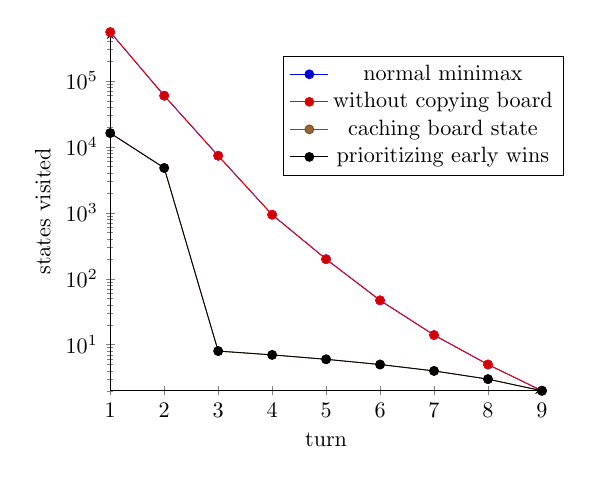
\begin{tikzpicture}[scale=.8]
        \begin{axis}[
            legend style={at={(.4,.6)},anchor=south west},
            axis lines = left,
            xlabel = turn,
            xtick = {0, 1, 2, 3, 4, 5, 6, 7, 8, 9},
            ymode = log,
            ylabel = states visited,
        ]
        \addplot+[
            mark=*,
        ] plot coordinates{
            (1,549946)
            (2,59705)
            (3,7332)
            (4,935)
            (5,198)
            (6,47)
            (7,14)
            (8,5)
            (9,2)
        };
        \addlegendentry{normal minimax}
        \addplot+[
            mark=*,
        ] plot coordinates{
            (1,549946)
            (2,59705)
            (3,7332)
            (4,935)
            (5,198)
            (6,47)
            (7,14)
            (8,5)
            (9,2)
        };
        \addlegendentry{without copying board}
        \addplot+[
            mark=*,
        ] plot coordinates{
            (1,16168)
            (2,4792)
            (3,8)
            (4,7)
            (5,6)
            (6,5)
            (7,4)
            (8,3)
            (9,2)
        };
        \addlegendentry{caching board state}
        \addplot+[
            mark=*,
        ] plot coordinates{
            (1,16168)
            (2,4792)
            (3,8)
            (4,7)
            (5,6)
            (6,5)
            (7,4)
            (8,3)
            (9,2)
        };
        \addlegendentry{prioritizing early wins}
        
        \end{axis}
    \end{tikzpicture}
\end{center}

In the first graph, we see a general exponential trend: as there are more open squares (at earlier moves), the time increases exponentially (reflecting that minimax trees are exponential in terms of the branching factor). Eliminating board copies slightly reduced the time, in proportion to how many moves were checked in the turn. Caching states reduced the time even more, and drastically after the first two turns (after which the rest of the game would already be cached). These later moves (3-9) are linear, as they depend merely on how many top-level moves (pre-cachced states) they need to check. Although it's impossible to tell with just two points, moves 1-2 are likely less-than exponential, as extrapolating along a linear form on the scaled graph would intersect the more-costly methods. That is, if the cache had been reset at each move, the graph would reflect this less-than exponential form (which makes sense, as branches would be removed from the tree). The last optimization actually slightly increased the time (a negligable amount), as taking depth into account adds constant time at each node.

The same exponential trend is shown in the states-visited graph for the original algorithms, as well as the sub-exponential trend for the cached methods. The only optimization that made a difference in terms of states, as expected, was caching the states.

\subsubsection{Minimax vs. Random}

When playing against a random agent, the minimax agent never loses, as the worst case scenario (seen in minimax vs. minimax games) for any optimal agent is a draw. Below is a chart of the winning percantages (from 100 games each) of minimax agent when playing as either the first or second player. Surprisingly, prioritizing earlier wins seems to increase the chance of a draw, which is likely an effect of the game not being deterministic (i.e., when the expected outcome is a draw, prioritizing early wins a few branches down happens to disfavor branches with more winning chances). As expected, the minimax agent going second reduces its likelihood of winning, as it has less moves and hence less control of the board.
\begin{center}

\scalebox{0.8}{
$
    \begin{array}{|c|c|c|}
        \hline
        & \textbf{minimax first} & \textbf{random first}\\
        \hline
        \textbf{no prioirty} & 99\% & 85\%\\
        \hline
        \textbf{prioritizing early wins} & 99\% & 76\%\\
        \hline
    \end{array}    
$
    }
\end{center}

The following graphs depicts the effect of prioritizing earlier wins. Games tend to be shorter, whether the minimax agent goes first or second, when it prioritizes earlier wins. Again, games last longer in general when going second, due to the fact that the 'o' player has less control of the board.

\begin{center}
    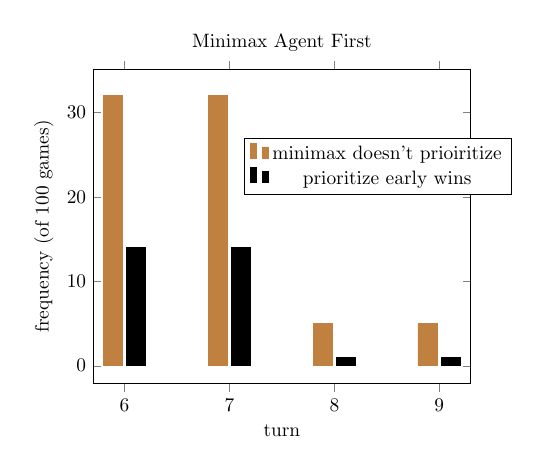
\begin{tikzpicture}[scale=.7]
        \begin{axis}[
            legend style={at={(.4,.6)},anchor=south west},
            ybar,
            xlabel = turn,
            ylabel = frequency (of 100 games),
            xtick = {6,7,8,9},
            title= Minimax Agent First
        ]
        %Below the red parabola is defined
        \addplot+[
            color = brown
        ]
        plot coordinates{
            (6,32)
            (7,32)
            (8,5)
            (9,5)
        };
        \addlegendentry{minimax doesn't prioiritize}

        \addplot+[
            color = black
        ]
        plot coordinates{
            (6,14)
            (7,14)
            (8,1)
            (9,1)
        };
        \addlegendentry{prioritize early wins}

        \end{axis}
    \end{tikzpicture}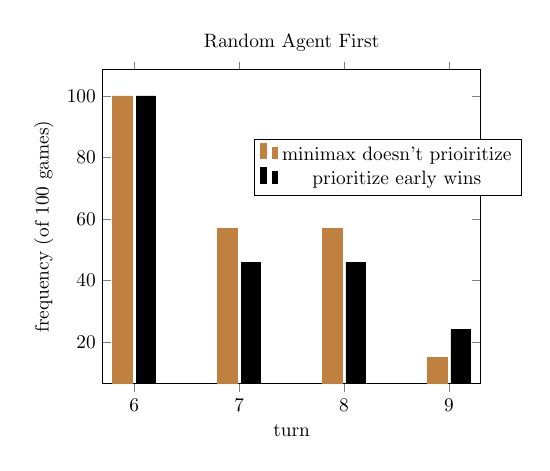
\begin{tikzpicture}[scale=.7]
        \begin{axis}[
            legend style={at={(.4,.6)},anchor=south west},
            ybar,
            xlabel = turn,
            xtick = {6,7,8,9},
            ylabel = frequency (of 100 games),
            title = Random Agent First
        ]
        %Below the red parabola is defined
        \addplot+[
            color = brown
        ]
        plot coordinates{
            (6,100)
            (7,57)
            (8,57)
            (9,15)
        };
        \addlegendentry{minimax doesn't prioiritize}

        \addplot+[
            color = black
        ]
        plot coordinates{
            (6,100)
            (7,46)
            (8,46)
            (9,24)
        };
        \addlegendentry{prioritize early wins}

        \end{axis}
    \end{tikzpicture}
\end{center}
